\documentclass[border=10pt]{standalone}
\usepackage{pgfplots}
\pgfplotsset{compat=1.18}
\begin{document}
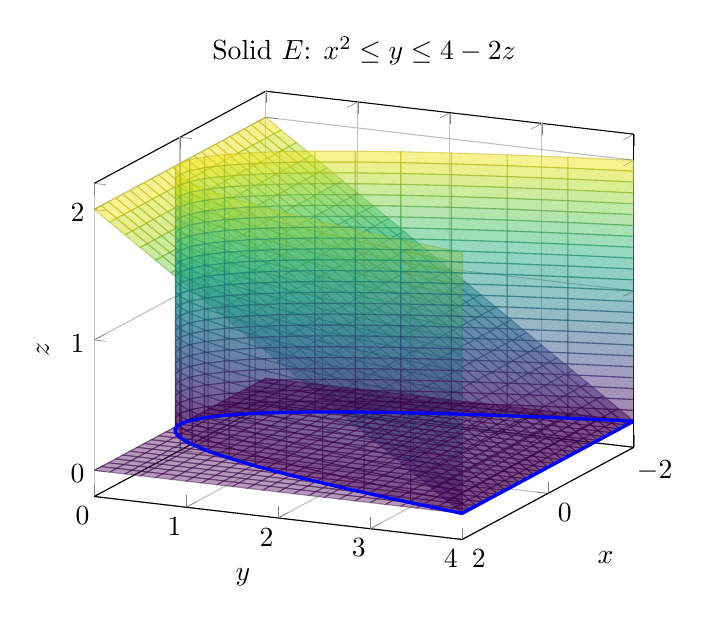
\begin{tikzpicture}
\begin{axis}[
    view={115}{18},
    xlabel={$x$}, ylabel={$y$}, zlabel={$z$},
    domain=-2:2, samples=25,
    y domain=0:2, samples y=25,
    title={Solid $E$: $x^2 \le y \le 4-2z$},
    colormap/viridis, grid]
% plane y = 4 - 2z
\addplot3[surf, opacity=0.5, domain=-2:2, y domain=0:2]
    ({x}, {4-2*y}, {y});
% parabolic cylinder y = x^2
\addplot3[surf, opacity=0.5, domain=-2:2, y domain=0:2]
    ({x}, {x^2}, {y});
% bottom z = 0 region inside parabola
\addplot3[surf, opacity=0.4, domain=-2:2, y domain=0:4]
    ({x}, {y}, {0});
% parabola silhouette on z=0
\addplot3[blue, very thick, domain=-2:2, samples=50]
    ({x}, {x^2}, {0});
\end{axis}
\end{tikzpicture}
\end{document}
